%% This file was auto-generated by IPython, do NOT edit
%% Conversion from the original notebook file:
%% IPython_notebook.ipynb
%%
\documentclass[11pt,english]{article}

%% This is the automatic preamble used by IPython.  Note that it does *not*
%% include a documentclass declaration, that is added at runtime to the overall
%% document.

\usepackage{amsmath}
\usepackage{amssymb}
\usepackage{graphicx}
\usepackage{ucs}
%% \usepackage[utf8x]{inputenc}

% needed for markdown enumerations to work
\usepackage{enumerate}

% Slightly bigger margins than the latex defaults
\usepackage{geometry}
\geometry{verbose,tmargin=3cm,bmargin=3cm,lmargin=2.5cm,rmargin=2.5cm}

% Define a few colors for use in code, links and cell shading
\usepackage{color}
\definecolor{orange}{cmyk}{0,0.4,0.8,0.2}
\definecolor{darkorange}{rgb}{.71,0.21,0.01}
\definecolor{darkgreen}{rgb}{.12,.54,.11}
\definecolor{myteal}{rgb}{.26, .44, .56}
\definecolor{gray}{gray}{0.45}
\definecolor{lightgray}{gray}{.95}
\definecolor{mediumgray}{gray}{.8}
\definecolor{inputbackground}{rgb}{.95, .95, .85}
\definecolor{outputbackground}{rgb}{.95, .95, .95}
\definecolor{traceback}{rgb}{1, .95, .95}

% Framed environments for code cells (inputs, outputs, errors, ...).  The
% various uses of \unskip (or not) at the end were fine-tuned by hand, so don't
% randomly change them unless you're sure of the effect it will have.
\usepackage{framed}

% remove extraneous vertical space in boxes
\setlength\fboxsep{0pt}

% codecell is the whole input+output set of blocks that a Code cell can
% generate.

% TODO: unfortunately, it seems that using a framed codecell environment breaks
% the ability of the frames inside of it to be broken across pages.  This
% causes at least the problem of having lots of empty space at the bottom of
% pages as new frames are moved to the next page, and if a single frame is too
% long to fit on a page, will completely stop latex from compiling the
% document.  So unless we figure out a solution to this, we'll have to instead
% leave the codecell env. as empty.  I'm keeping the original codecell
% definition here (a thin vertical bar) for reference, in case we find a
% solution to the page break issue.

%% \newenvironment{codecell}{%
%%     \def\FrameCommand{\color{mediumgray} \vrule width 1pt \hspace{5pt}}%
%%    \MakeFramed{\vspace{-0.5em}}}
%%  {\unskip\endMakeFramed}

% For now, make this a no-op...
\newenvironment{codecell}{}

 \newenvironment{codeinput}{%
   \def\FrameCommand{\colorbox{inputbackground}}%
   \MakeFramed{\advance\hsize-\width \FrameRestore}}
 {\unskip\endMakeFramed}

\newenvironment{codeoutput}{%
   \def\FrameCommand{\colorbox{outputbackground}}%
   \vspace{-1.4em}
   \MakeFramed{\advance\hsize-\width \FrameRestore}}
 {\unskip\medskip\endMakeFramed}

\newenvironment{traceback}{%
   \def\FrameCommand{\colorbox{traceback}}%
   \MakeFramed{\advance\hsize-\width \FrameRestore}}
 {\endMakeFramed}

% Use and configure listings package for nicely formatted code
\usepackage{listingsutf8}
\lstset{
  language=python,
  inputencoding=utf8x,
  extendedchars=\true,
  aboveskip=\smallskipamount,
  belowskip=\smallskipamount,
  xleftmargin=2mm,
  breaklines=true,
  basicstyle=\small \ttfamily,
  showstringspaces=false,
  keywordstyle=\color{blue}\bfseries,
  commentstyle=\color{myteal},
  stringstyle=\color{darkgreen},
  identifierstyle=\color{darkorange},
  columns=fullflexible,  % tighter character kerning, like verb
}

% The hyperref package gives us a pdf with properly built
% internal navigation ('pdf bookmarks' for the table of contents,
% internal cross-reference links, web links for URLs, etc.)
\usepackage{hyperref}
\hypersetup{
  breaklinks=true,  % so long urls are correctly broken across lines
  colorlinks=true,
  urlcolor=blue,
  linkcolor=darkorange,
  citecolor=darkgreen,
  }

% hardcode size of all verbatim environments to be a bit smaller
\makeatletter
\g@addto@macro\@verbatim\small\topsep=0.5em\partopsep=0pt
\makeatother

% Prevent overflowing lines due to urls and other hard-to-break entities.
\sloppy

\begin{document}

\section{A brief tour of the IPython notebook}

This document will give you a brief tour of the capabilities of the
IPython notebook.

This IPython notebook is a modification of a notebook from an
\href{https://github.com/ipython/ipython-in-depth/tree/master/notebooks}{IPython
tutorial}

\subsection{How many of you have used IPython before?}


The first thing you need to know is that you are still controlling the
same old IPython you're used to, so things like shell aliases and magic
commands still work:

\begin{codecell}
\begin{codeinput}
\begin{lstlisting}
# Tab completion
from numpy import absolute
\end{lstlisting}
\end{codeinput}
\end{codecell}
\begin{codecell}
\begin{codeinput}
\begin{lstlisting}
# Explore your objects
def square(n):
    """Square n and return it's value
    """
    return n**2

square?
square??
\end{lstlisting}
\end{codeinput}
\end{codecell}
\begin{codecell}
\begin{codeinput}
\begin{lstlisting}
ls
\end{lstlisting}
\end{codeinput}
\begin{codeoutput}
\begin{verbatim}
IPython_notebook.ipynb  llvm.ipynb
\end{verbatim}
\end{codeoutput}
\end{codecell}
\begin{codecell}
\begin{codeinput}
\begin{lstlisting}
pwd
\end{lstlisting}
\end{codeinput}
\begin{codeoutput}
\begin{verbatim}
u'/home/punchagan/software/my-repos/talks/pycon-2012-scipy-kids'
\end{verbatim}
\end{codeoutput}
\end{codecell}
\begin{codecell}
\begin{codeinput}
\begin{lstlisting}
foo = !ls
print foo
\end{lstlisting}
\end{codeinput}
\begin{codeoutput}
\begin{verbatim}
['IPython_notebook.ipynb', 'llvm.ipynb', 'lnum.py', 'media', 'new_scipy_kids.org', 'Pandas.ipynb', 'PyPy.ipynb', 'sachin-odi-year.csv', 'scikits.ipynb']
\end{verbatim}
\end{codeoutput}
\end{codecell}
\begin{codecell}
\begin{codeinput}
\begin{lstlisting}
# Shell commands
!ping in.pycon.org -c 3
\end{lstlisting}
\end{codeinput}
\begin{codeoutput}
\begin{verbatim}
PING pycon.anandology.com (106.187.46.141) 56(84) bytes of data.
\end{verbatim}
\begin{verbatim}
64 bytes from linode.futurelabs.in (106.187.46.141): icmp_req=1 ttl=50 time=654 ms
\end{verbatim}
\begin{verbatim}
64 bytes from linode.futurelabs.in (106.187.46.141): icmp_req=2 ttl=50 time=397 ms
\end{verbatim}
\begin{verbatim}
64 bytes from linode.futurelabs.in (106.187.46.141): icmp_req=3 ttl=50 time=511 ms

--- pycon.anandology.com ping statistics ---
3 packets transmitted, 3 received, 0% packet loss, time 1999ms
rtt min/avg/max/mdev = 397.908/521.202/654.140/104.831 ms
\end{verbatim}
\end{codeoutput}
\end{codecell}
\subsection{Plots with matplotlib}
IPython adds an `inline' matplotlib backend, which embeds any matplotlib
figures into the notebook.

\begin{codecell}
\begin{codeinput}
\begin{lstlisting}
%pylab inline
\end{lstlisting}
\end{codeinput}
\end{codecell}
\begin{codecell}
\begin{codeinput}
\begin{lstlisting}
x = linspace(0, 3*pi, 500)
plot(x, sin(x**2))
title('A simple chirp');
\end{lstlisting}
\end{codeinput}
\end{codecell}
You can paste blocks of input with prompt markers, such as those from
\href{http://docs.python.org/tutorial/interpreter.html\#interactive-mode}{the
official Python tutorial}

\begin{codecell}
\begin{codeinput}
\begin{lstlisting}
>>> the_world_is_flat = 1
>>> if the_world_is_flat:
...     print "Be careful not to fall off!"
\end{lstlisting}
\end{codeinput}
\end{codecell}
Errors are shown in informative ways:

\begin{codecell}
\begin{codeinput}
\begin{lstlisting}
%run /tmp/foo.py
\end{lstlisting}
\end{codeinput}
\begin{codeoutput}
\begin{verbatim}
ERROR: File `u'/tmp/foo.py'` not found.
\end{verbatim}
\end{codeoutput}
\end{codecell}
\begin{codecell}
\begin{codeinput}
\begin{lstlisting}
x = 1
y = 4
z = y/(1-x)
\end{lstlisting}
\end{codeinput}
\end{codecell}
When IPython needs to display additional information (such as providing
details on an object via \texttt{x?} it will automatically invoke a
pager at the bottom of the screen:

\begin{codecell}
\begin{codeinput}
\begin{lstlisting}
magic
\end{lstlisting}
\end{codeinput}
\end{codecell}
\subsection{Non-blocking output of kernel}

If you execute the next cell, you will see the output arriving as it is
generated, not all at the end.

\begin{codecell}
\begin{codeinput}
\begin{lstlisting}
import time, sys
for i in range(8):
    print i,
    time.sleep(0.5)
\end{lstlisting}
\end{codeinput}
\begin{codeoutput}
\begin{verbatim}
0
\end{verbatim}
\begin{verbatim}
1
\end{verbatim}
\begin{verbatim}
2
\end{verbatim}
\begin{verbatim}
3
\end{verbatim}
\begin{verbatim}
4
\end{verbatim}
\begin{verbatim}
5
\end{verbatim}
\begin{verbatim}
6
\end{verbatim}
\begin{verbatim}
7
\end{verbatim}
\end{codeoutput}
\end{codecell}
\subsection{Clean crash and restart}

We call the low-level system libc.time routine with the wrong argument
via ctypes to segfault the Python interpreter:

\begin{codecell}
\begin{codeinput}
\begin{lstlisting}
import sys
from ctypes import CDLL
# This will crash a Linux or Mac system; equivalent calls can be made on Windows
dll = 'dylib' if sys.platform == 'darwin' else 'so.6'
libc = CDLL("libc.%s" % dll)
libc.time(-1)  # BOOM!!
\end{lstlisting}
\end{codeinput}
\end{codecell}
\subsection{Markdown cells can contain formatted text and code}

You can \emph{italicize}, \textbf{boldface}

\begin{itemize}
\item
  build
\item
  lists
\end{itemize}
and embed code meant for illustration instead of execution in Python:

\begin{verbatim}
def f(x):
    """a docstring"""
    return x**2
\end{verbatim}
or other languages:

\begin{verbatim}
if (i=0; i<n; i++) {
  printf("hello %d\n", i);
  x += 4;
}
\end{verbatim}


Courtesy of MathJax, you can include mathematical expressions both
inline: $e^{i\pi} + 1 = 0$ and displayed:

\[e^x=\sum_{i=0}^\infty \frac{1}{i!}x^i\]

\subsection{Rich displays: include anyting a browser can show}

Note that we have an actual protocol for this, see the
\texttt{display\_protocol} notebook for further details.

\subsubsection{Images}


\begin{codecell}
\begin{codeinput}
\begin{lstlisting}
from IPython.display import Image
Image(filename='media/logo.jpg')
\end{lstlisting}
\end{codeinput}
\begin{codeoutput}
\begin{verbatim}
<IPython.core.display.Image object at 0x3552b10>
\end{verbatim}
\end{codeoutput}
\end{codecell}
An image can also be displayed from raw data or a url

\begin{codecell}
\begin{codeinput}
\begin{lstlisting}
Image(url='http://python.org/images/python-logo.gif')
\end{lstlisting}
\end{codeinput}
\end{codecell}
SVG images are also supported out of the box (since modern browsers do a
good job of rendering them):

\begin{codecell}
\begin{codeinput}
\begin{lstlisting}
from IPython.display import SVG
SVG(filename='media/python-logo.svg')
\end{lstlisting}
\end{codeinput}
\begin{codeoutput}
\begin{verbatim}
<IPython.core.display.SVG object at 0x3ced350>
\end{verbatim}
\end{codeoutput}
\end{codecell}
\subsubsection{Video}


And more exotic objects can also be displayed, as long as their
representation supports the IPython display protocol.

For example, videos hosted externally on YouTube are easy to load (and
writing a similar wrapper for other hosted content is trivial):

\begin{codecell}
\begin{codeinput}
\begin{lstlisting}
from IPython.display import YouTubeVideo
# a talk about IPython at Sage Days at U. Washington, Seattle.
# Video credit: William Stein.
YouTubeVideo('1j_HxD4iLn8')
\end{lstlisting}
\end{codeinput}
\begin{codeoutput}
\begin{verbatim}
<IPython.lib.display.YouTubeVideo at 0x2dba8d0>
\end{verbatim}
\end{codeoutput}
\end{codecell}
Using the nascent video capabilities of modern browsers, you may also be
able to display local videos. At the moment this doesn't work very well
in all browsers, so it may or may not work for you; we will continue
testing this and looking for ways to make it more robust.

The following cell loads a local file called \texttt{animation.m4v},
encodes the raw video as base64 for http transport, and uses the HTML5
video tag to load it. On Chrome 15 it works correctly, displaying a
control bar at the bottom with a play/pause button and a location
slider.

\begin{codecell}
\begin{codeinput}
\begin{lstlisting}
from IPython.display import HTML
video = open("media/animation.webm", "rb").read()
video_encoded = video.encode("base64")
video_tag = '<video controls alt="test" src="data:video/webm;base64,{0}">'.format(video_encoded)
HTML(data=video_tag)
\end{lstlisting}
\end{codeinput}
\begin{codeoutput}
\begin{verbatim}
<IPython.core.display.HTML object at 0x3ced0d0>
\end{verbatim}
\end{codeoutput}
\end{codecell}
\subsection{Local Files}

The above examples embed images and video from the notebook filesystem
in the output areas of code cells. It is also possible to request these
files directly in markdown cells if they reside in the notebook
directory via relative urls prefixed with \texttt{files/}:

\begin{verbatim}
files/[subdirectory/]<filename>
\end{verbatim}
For example, in the example notebook folder, we have the Python logo,
addressed as:

\begin{verbatim}
<img src="media/python-logo.svg" />
\end{verbatim}
and a video with the HTML5 video tag:

\begin{verbatim}
<video controls src="files/media/animation.webm" />
\end{verbatim}
These do not embed the data into the notebook file, and require that the
files exist when you are viewing the notebook.

\subsubsection{Security of local files}

Note that this means that the IPython notebook server also acts as a
generic file server for files inside the same tree as your notebooks.
Access is not granted outside the notebook folder so you have strict
control over what files are visible, but for this reason it is highly
recommended that you do not run the notebook server with a notebook
directory at a high level in your filesystem (e.g.~your home directory).

When you run the notebook in a password-protected manner, local file
access is restricted to authenticated users unless read-only views are
active.

\subsubsection{External sites}

You can even embed an entire page from another site in an iframe; for
example this is today's Wikipedia page for mobile users:

\begin{codecell}
\begin{codeinput}
\begin{lstlisting}
HTML('<iframe src=http://in.pycon.org/#schedule width=700 height=350>')
\end{lstlisting}
\end{codeinput}
\begin{codeoutput}
\begin{verbatim}
<IPython.core.display.HTML object at 0x3552b50>
\end{verbatim}
\end{codeoutput}
\end{codecell}
\section{Loading external codes}

\begin{itemize}
\item
  Drag and drop a \texttt{.py} in the dashboard
\item
  Use \texttt{\%load} with any local or remote url:
  \href{http://matplotlib.sourceforge.net/gallery.html}{the Matplotlib
  Gallery!}
\end{itemize}
In this notebook we've kept the output saved so you can see the result,
but you should run the next cell yourself (with an active internet
connection).

Let's make sure we have pylab again, in case we have restarted the
kernel due to the crash demo above

\begin{codecell}
\begin{codeinput}
\begin{lstlisting}
%pylab inline
\end{lstlisting}
\end{codeinput}
\end{codecell}
\begin{codecell}
\begin{codeinput}
\begin{lstlisting}
%load http://matplotlib.sourceforge.net/mpl_examples/pylab_examples/integral_demo.py
\end{lstlisting}
\end{codeinput}
\end{codecell}
\begin{codecell}
\begin{codeinput}
\begin{lstlisting}
#!/usr/bin/env python

# implement the example graphs/integral from pyx
from pylab import *
from matplotlib.patches import Polygon

def func(x):
    return (x-3)*(x-5)*(x-7)+85

ax = subplot(111)

a, b = 2, 9 # integral area
x = arange(0, 10, 0.01)
y = func(x)
plot(x, y, linewidth=1)

# make the shaded region
ix = arange(a, b, 0.01)
iy = func(ix)
verts = [(a,0)] + zip(ix,iy) + [(b,0)]
poly = Polygon(verts, facecolor='0.8', edgecolor='k')
ax.add_patch(poly)

text(0.5 * (a + b), 30,
     r"$\int_a^b f(x)\mathrm{d}x$", horizontalalignment='center',
     fontsize=20)

axis([0,10, 0, 180])
figtext(0.9, 0.05, 'x')
figtext(0.1, 0.9, 'y')
ax.set_xticks((a,b))
ax.set_xticklabels(('a','b'))
ax.set_yticks([])
show()

\end{lstlisting}
\end{codeinput}
\end{codecell}
\subsection{Mathematics and SymPy support}

And we also support the display of mathematical expressions typeset in
LaTeX, which is rendered in the browser thanks to the
\href{http://mathjax.org}{MathJax library}.

Note that this is \emph{different} from the above examples. Above we
were typing mathematical expressions in Markdown cells (along with
normal text) and letting the browser render them; now we are displaying
the output of a Python computation as a LaTeX expression wrapped by the
\texttt{Math()} object so the browser renders it. The \texttt{Math}
object will add the needed LaTeX delimiters (\texttt{\$\$}) if they are
not provided:

\begin{codecell}
\begin{codeinput}
\begin{lstlisting}
from IPython.display import Math
Math(r'F(k) = \int_{-\infty}^{\infty} f(x) e^{2\pi i k} dx')
\end{lstlisting}
\end{codeinput}
\end{codecell}
With the \texttt{Latex} class, you have to include the delimiters
yourself. This allows you to use other LaTeX modes such as
\texttt{eqnarray}:

\begin{codecell}
\begin{codeinput}
\begin{lstlisting}
from IPython.display import Latex
Latex(r"""\begin{eqnarray}
\nabla \times \vec{\mathbf{B}} -\, \frac1c\, \frac{\partial\vec{\mathbf{E}}}{\partial t} & = \frac{4\pi}{c}\vec{\mathbf{j}} \\
\nabla \cdot \vec{\mathbf{E}} & = 4 \pi \rho \\
\nabla \times \vec{\mathbf{E}}\, +\, \frac1c\, \frac{\partial\vec{\mathbf{B}}}{\partial t} & = \vec{\mathbf{0}} \\
\nabla \cdot \vec{\mathbf{B}} & = 0
\end{eqnarray}""")
\end{lstlisting}
\end{codeinput}
\end{codecell}
Using these tools, we can integrate with the
\href{http://sympy.org}{SymPy} package to perform symbolic
manipulations, and combined with numpy and matplotlib, also displays
numerical visualizations of symbolically constructed expressions.

We first load sympy printing and plotting support, as well as all of
sympy:

\begin{codecell}
\begin{codeinput}
\begin{lstlisting}
%load_ext sympyprinting
%pylab inline

from __future__ import division
import sympy as sym
from sympy import *
x, y, z = symbols("x y z")
k, m, n = symbols("k m n", integer=True)
f, g, h = map(Function, 'fgh')
\end{lstlisting}
\end{codeinput}
\begin{codeoutput}
\begin{verbatim}
Welcome to pylab, a matplotlib-based Python environment [backend: module://IPython.zmq.pylab.backend_inline].
For more information, type 'help(pylab)'.
\end{verbatim}
\end{codeoutput}
\end{codecell}
Elementary operations

\begin{codecell}
\begin{codeinput}
\begin{lstlisting}
Rational(3,2)*pi + exp(I*x) / (x**2 + y)
\end{lstlisting}
\end{codeinput}
\begin{codeoutput}
$
$
\
f
r
a
c
{
3
}
{
2
}

\
p
i

+

\
f
r
a
c
{
e
^
{
\
m
a
t
h
b
f
{
\
i
m
a
t
h
}

x
}
}
{
x
^
{
2
}

+

y
}
$
$
\begin{verbatim}

        ⅈ⋅x
3⋅π    ℯ
─── + ──────
 2     2
      x  + y
\end{verbatim}
\end{codeoutput}
\end{codecell}
\begin{codecell}
\begin{codeinput}
\begin{lstlisting}
exp(I*x).subs(x,pi).evalf()
\end{lstlisting}
\end{codeinput}
\begin{codeoutput}
$
$
-
1
.
0
$
$
\begin{verbatim}
-1.00000000000000
\end{verbatim}
\end{codeoutput}
\end{codecell}
\begin{codecell}
\begin{codeinput}
\begin{lstlisting}
exp(pi * sqrt(163)).evalf(50)
\end{lstlisting}
\end{codeinput}
\begin{codeoutput}
$
$
2
6
2
5
3
7
4
1
2
6
4
0
7
6
8
7
4
3
.
9
9
9
9
9
9
9
9
9
9
9
9
2
5
0
0
7
2
5
9
7
1
9
8
1
8
5
6
8
8
8
8
$
$
\begin{verbatim}
262537412640768743.99999999999925007259719818568888
\end{verbatim}
\end{codeoutput}
\end{codecell}
\section{Cell magics}


\begin{codecell}
\begin{codeinput}
\begin{lstlisting}
%lsmagic
\end{lstlisting}
\end{codeinput}
\begin{codeoutput}
\begin{verbatim}
Available line magics:
%alias  %alias_magic  %autocall  %automagic  %bookmark  %cd  %clear  %colors  %config  %connect_info  %debug  %dhist  %dirs  %doctest_mode  %ed  %edit  %env  %gui  %hist  %history  %install_default_config  %install_ext  %install_profiles  %killbgscripts  %less  %load  %load_ext  %loadpy  %logoff  %logon  %logstart  %logstate  %logstop  %lsmagic  %macro  %magic  %man  %more  %notebook  %page  %pastebin  %pdb  %pdef  %pdoc  %pfile  %pinfo  %pinfo2  %popd  %pprint  %precision  %profile  %prun  %psearch  %psource  %pushd  %pwd  %pycat  %pylab  %qtconsole  %quickref  %recall  %rehashx  %reload_ext  %rep  %rerun  %reset  %reset_selective  %run  %save  %sc  %store  %sx  %system  %tb  %time  %timeit  %unalias  %unload_ext  %who  %who_ls  %whos  %xdel  %xmode

Available cell magics:
%%!  %%bash  %%capture  %%file  %%javascript  %%latex  %%perl  %%prun  %%ruby  %%script  %%sh  %%svg  %%sx  %%system  %%timeit

Automagic is ON, % prefix IS NOT needed for line magics.
\end{verbatim}
\begin{verbatim}

\end{verbatim}
\end{codeoutput}
\end{codecell}
\begin{codecell}
\begin{codeinput}
\begin{lstlisting}
%pylab inline
\end{lstlisting}
\end{codeinput}
\begin{codeoutput}
\begin{verbatim}
Welcome to pylab, a matplotlib-based Python environment [backend: module://IPython.zmq.pylab.backend_inline].
For more information, type 'help(pylab)'.
\end{verbatim}
\end{codeoutput}
\end{codecell}
\begin{codecell}
\begin{codeinput}
\begin{lstlisting}
%timeit np.linalg.eigvals(np.random.rand(100,100))
\end{lstlisting}
\end{codeinput}
\begin{codeoutput}
\begin{verbatim}
1 loops, best of 3: 11.3 ms per loop
\end{verbatim}
\end{codeoutput}
\end{codecell}
\begin{codecell}
\begin{codeinput}
\begin{lstlisting}
%%timeit a = np.random.rand(100, 100)
np.linalg.eigvals(a)
\end{lstlisting}
\end{codeinput}
\begin{codeoutput}
\begin{verbatim}
100 loops, best of 3: 6.8 ms per loop
\end{verbatim}
\end{codeoutput}
\end{codecell}
\begin{codecell}
\begin{codeinput}
\begin{lstlisting}
%%script lnum.py
first line
second line
more lines
\end{lstlisting}
\end{codeinput}
\begin{codeoutput}
\begin{verbatim}
0 : first line
1 : second line
2 : more lines
\end{verbatim}
\end{codeoutput}
\end{codecell}
\begin{codecell}
\begin{codeinput}
\begin{lstlisting}
%%bash
echo $BASH
\end{lstlisting}
\end{codeinput}
\begin{codeoutput}
\begin{verbatim}
/bin/bash
\end{verbatim}
\end{codeoutput}
\end{codecell}
IPython has an \texttt{rmagic} extension that contains a some magic
functions for working with R via rpy2. This extension can be loaded
using the \texttt{\%load\_ext} magic as follows:

\begin{codecell}
\begin{codeinput}
\begin{lstlisting}
%load_ext rmagic
\end{lstlisting}
\end{codeinput}
\end{codecell}
Let's plot a simple scatter plot using both matplotlib and R.

\begin{codecell}
\begin{codeinput}
\begin{lstlisting}
import numpy as np
import pylab
X = np.array([0,1,2,3,4])
Y = np.array([3,5,4,6,7])
pylab.scatter(X, Y)
del _17
\end{lstlisting}
\end{codeinput}
\begin{codeoutput}
\begin{center}
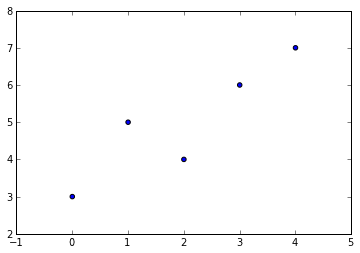
\includegraphics[width=6in]{IPython_notebook_files/IPython_notebook_fig_00.png}
\par
\end{center}
\begin{verbatim}
Figure(480x320)
\end{verbatim}
\end{codeoutput}
\end{codecell}
\begin{codecell}
\begin{codeinput}
\begin{lstlisting}
%Rpush X Y
v1 = %R plot(X,Y); print(summary(lm(Y~X))); vv=mean(X)*mean(Y)
print 'v1 is:', v1
v2 = %R mean(X)*mean(Y)
print 'v2 is:', v2
\end{lstlisting}
\end{codeinput}
\begin{codeoutput}
\begin{verbatim}
Call:
lm(formula = Y ~ X)

Residuals:
   1    2    3    4    5
-0.2  0.9 -1.0  0.1  0.2

Coefficients:
            Estimate Std. Error t value Pr(>|t|)
(Intercept)   3.2000     0.6164   5.191   0.0139 *
X             0.9000     0.2517   3.576   0.0374 *
---
Signif. codes:  0 ‘***’ 0.001 ‘**’ 0.01 ‘*’ 0.05 ‘.’ 0.1 ‘ ’ 1

Residual standard error: 0.7958 on 3 degrees of freedom
Multiple R-squared:  0.81,	Adjusted R-squared: 0.7467
F-statistic: 12.79 on 1 and 3 DF,  p-value: 0.03739
\end{verbatim}
\begin{center}
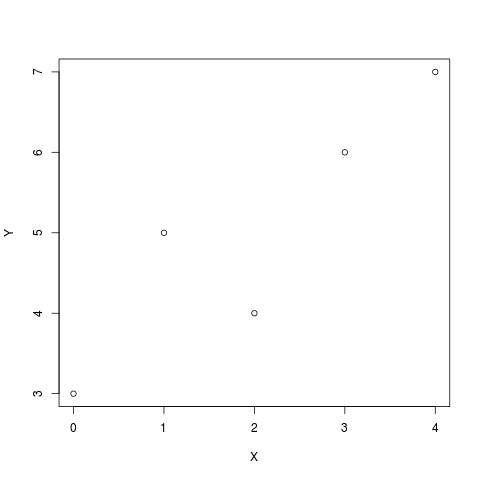
\includegraphics[width=6in]{IPython_notebook_files/IPython_notebook_fig_01.png}
\par
\end{center}
\begin{verbatim}
v1 is: [ 10.]
v2 is: [ 10.]
\end{verbatim}
\end{codeoutput}
\end{codecell}

\end{document}
